\chapter{Implementação}
\label{cap5}

Este capítulo visa expressar o funcionamento prático dos microsserviços implementados.
%
Isto é necessário, tal que a escolha da linguagem, tecnologias utilizadas e boas práticas adotadas em seu desenvolvimento interferem a qualidade do serviço desenvolvido.

Devido a preocupação das bibliotecas disponíveis para utilização e as linguagens de programação que permitem utilizar tais tecnologias,
a Seção~\ref{sec:tecnologias} descreve a necessidade tecnológica necessária para o desenvolvimento. A partir desta demanda funcional, mostra-se qual linguagem de programação utilizar e por sua vez, o conjunto de bibliotecas ou serviços externos que derivam de tal escolha.
%
Não derivado diretamente da linguagem escolhida, porém tendo uma correlação forte desta escolha, a Seção~\ref{sec:tecnologias} também aborda o conjunto de serviços externos utilizados para facilitar o desenvolvimento e implantação dos microsserviços.

Por fim, para contextualizar o funcionamento dos microsserviços operando em rede, a Seção~\ref{sec:interconexao} visa descrever a interconexão dos microsserviços implementados.

\section{Tecnologias Utilizadas}
\label{sec:tecnologias}

A seleção do conjunto de tecnologias que estaram em execução durante o momento dos testes é importante, visto que eles implicam diretamente no desempenho e consumo de recursos das arquiteturas selecionadas.
%
Por este motivo, esta sessão definirá qual o conjunto tecnologico utilizado no desenvolvimento das arquiteturas propostas.

Inicialmente existe uma preocupação com a linguagem de programação utilizada, visto que ela precisa ter um bom desempenho com programação paralela e, ao mesmo tempo, conter bibliotecas que auxiliem o desenvolvimento rápido de tais serviços.
%
Neste sentido, foi levantado um conjunto de linguagens de programação a qual viabilizassem o projeto, seguindo os seguintes critérios:

\begin{itemize}
  \item Desempenho de programas paralelos
  \item Facilidade de escrita de código
  \item Bibliotecas para conexão com banco de dados, tanto para dados permanentes quanto dados temporários
  \item Escrita de serviços \ac{rpc}
  \item Escrita de serviços \ac{web}
  \item Linguagem compilada ou interpretada
  \item Linguagem tipada ou dinâmica
\end{itemize}

A partir destes critérios, a linguagem selecionada foi Golang, por se tratar de uma linguagem a qual possuo domínio e enquadra-se nos critérios definidos.
%
Outro critério implícito para o desenvolvimento é a homogenidade da linguagem de programação em todos os microsserviços, na qual utilizar apenas uma única linguagem trás o benefício de escrever o núcleo de regras de negócio somente uma única vez, sem repeti-lo sem diversos pontos dos serviços.

Desta forma, temos uma linguagem de desempenho compatível a viabilizar o projeto, a qual permite escrever as regras de negócio em um único ponto central reaproveitando trechos de código existentes entre vários microsserviços.

Por fim, utilizando a Linguagem GoLang pode-se utilizar diversas bibliotecas diferentes. Por este motivo, também se faz de interesse definir quais bibliotecas foram utilizadas para o desenvolvimento das arquiteturas de microsserviços para jogos \ac{mmorpg}.

As principais bibliotecas utilizadas foram:

\begin{itemize}
  \item gin: Servidor Web para serviços de alto desempenho. O seu principal foco é servir uma interface de comunicação com \ac{api}, utilizando dados no formato \ac{xml} ou \ac{json}.
  \item gorm: Trata-se de uma biblioteca de objetos relacionais, a qual suporta conexão direta ao banco PostgreSQL.
  \item go-redis: Trata-se de uma biblioteca a qual facilita a leitura e escrita de dados em bancos de dados em memória.
  \item net/rpc: Trata-se de uma biblioteca padrão da linguagem Go para escrita de serviços \ac{rpc}.
\end{itemize}

Tais bibliotecas descritas foram utilizadas em todas as arquiteturas, seguindo o padrão de interface \ac{rpc} e Web a qual são utilizados para acesso aos serviços de rede.

Não somente a linguagem Go e as bibliotecas utilizadas são importantes para definir o fluxo de implementação das arquiteturas.
%
Foi utilizado um fluxo de desenvolvimento contínuo a partir do \textit{Github}, utilizando a ferramenta \textit{TravisCI} para executar testes automatizados. Estes testes executavam chamadas ao serviços, esperando uma resposta coerente ao esperado. O mesmo também obtinha métricas de porcentagem de código coberto, enviando para o Coveralls.
%
Ao fim dos testes, as arquiteturas eram automaticamente publicadas no \textit{DockerHub}, como imagens de contâinerer \textit{Docker}.

Este fluxo garantiu a qualidade das aplicações durante a implementação, realizando testes e construindo a aplicação, sendo um papel similar aos serviços de construção e implantação demonstrado na arquitetura Willson.

Após definir o arcabolço tecnológico utilizado, faz-se necessário descrever o ambiente distribuído desenvolvido, a fim de garantir uma melhor visibilidade dos microsserviços implementados.

\section{Interconexão entre os microsserviços}
\label{sec:interconexao}

Ao todo foram implementados 11 microsserviços, a qual possuem conexão entre sí, com os bancos de dados e os seus respectivos clientes, tal qual a definição das arquiteturas selecionadas descreve.
%
Por este motivo, torna-se interessante descrever a interconexão entre os microsserviços e exibir o modelo de comunicação entre estes serviços desenvolvidos.

A arquitetura Rudy contém um microsserviço especial intermediário para conexão com o banco de dados.
%
O seu principal objetivo é concentrar todas as chamadas para o banco de dados, minimizando erros de acesso ao banco de dados.
%
Esta característica especial é visível na Figura~\ref{fig:interconexao_rudy}.

\begin{figure}[htb!]
  \caption{Interconexões da arquitetura Rudy.}
  \label{fig:interconexao_rudy}
  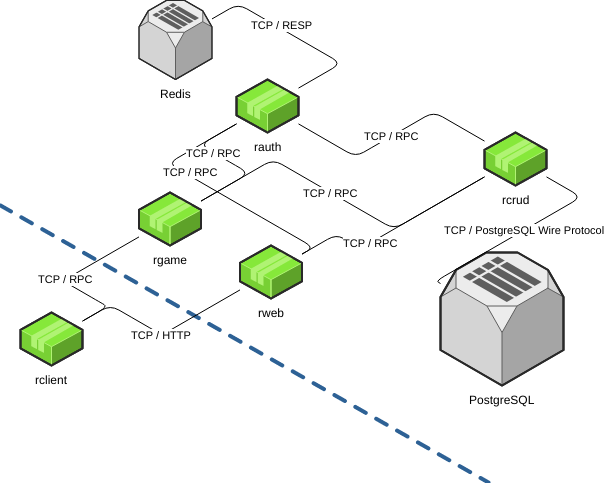
\includegraphics[width=0.8\textwidth]{figuras/interconexoes/rudy.png}
  \centering

  Fonte: O próprio autor.
\end{figure}

Conforme visível na Figura~\ref{fig:interconexao_rudy}, existe uma camada a mais interceptando o acesso ao banco, a qual espera-se aumentar o tempo de resposta de requisições ao acessar dados.

Na arquitetura Salz as conexões com o banco são diretas a partir dos microsserviços, sem a utilização de um microsserviço intermediário.
%
Além desta característica, a arquitetura Salz divide o microsserviço de jogo entre o Chat e Jogo. Esta abstração tende a reduzir o consumo de recursos de uma instância, permitindo mais conexões simultâneas sem estressar o serviço de jogo.
%
Ela pode ser observada na Figura~\ref{fig:interconexao_salz}

\begin{figure}[htb!]
  \caption{Interconexões da arquitetura Salz.}
  \label{fig:interconexao_salz}
  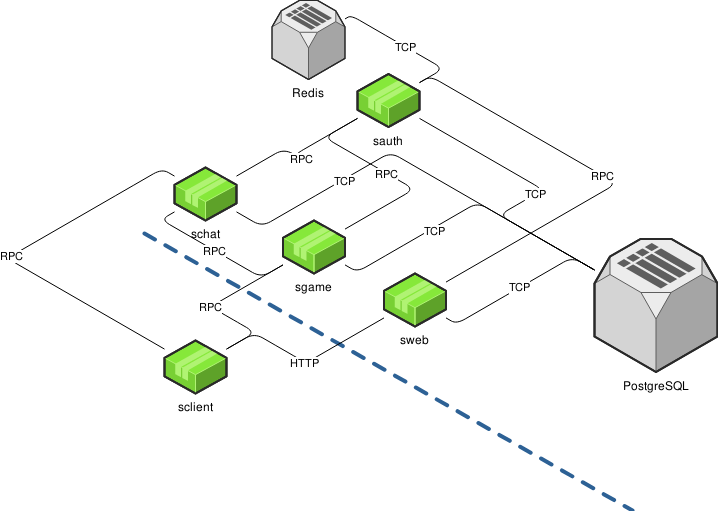
\includegraphics[width=0.8\textwidth]{figuras/interconexoes/salz.png}
  \centering

  Fonte: O próprio autor.
\end{figure}
